\chapter{Projeto de Controlador com Alocação de Polos Baseado nos Modelos Identificados} \label{cap5}
Com o sistema identificado, podemos finalmente controlá-l, faremos isso através de realimentação de estados para o modelo identificado por subespaços e para o modelo identificado por mínimos quadrados nesta seção.
\section{Alocação de Polos com Realimentação de Estados}
Primeiramente precisamos passar o modelo identificado por mínimos quadrados de ARX para espaço de estado. Fazemos isso usando a função do Matlab tf2ss, onde entramos com o nominador e denominador do modelo ARX e a função nos retorna as matrizes A, B, C e D do sistema em espaço de estados. O modelo obtido por espaço de estados será chamado de modelo 1 e o modelo obtido por mínimos quadrados será chamado de modelo 2.


Desejamos controlar os dois modelos utilizando alocação de polos com realimentação de estados. Projetamos o controlador para que o sistema tenha um sobrevalor menor que 4\% do seu valor final e um tempo de assentamento menor que 2 segundos. Previamente foi escolhido um tempo de assentamento menor que 1 segundo mas foi constatado que o ganho necessário para tanto excedia os limites de atuação segura da turbina RC presente no sistema.

\subsection{Modelo 1: Identificado por Subespaços}

Para atender esses requisitos de tempo de assentamento $t_s<2 ~s$ e sobrevalor máximo de $ovs<4\%$ calculamos os valores de $\zeta$ e $\omega_n$ usados na equação característica de um sistema de segunda ordem \eqref{eq:mso}, usando as equações \eqref{eq:ovs} e \eqref{eq:ts}.

\begin{equation}\label{eq:mso}
G(s)=\dfrac{\omega_n^2}{s^2+2 \zeta \omega_n  s+ \omega_n^2}
\end{equation}

\begin{equation}\label{eq:ovs}
ovs=e^{\dfrac{\zeta \pi}{\sqrt{1-\zeta^2}}}<4\%
\end{equation}

\begin{equation}\label{eq:ts}
t_s=\dfrac{4}{\zeta \omega_n}<2~s
\end{equation}

Encontramos $\zeta>0.7157$ e $\omega_n>2.7945$, e escolhemos os valores de $\zeta=0.9$ e $\omega_n=3$. Ao aplicar esses valores na equação \eqref{eq:mso} obtemos os polos que precisamos alocar no domínio s, $s_1=-2.7+1.3077 i$ e $s_2=-2.7-1.3077i$. Como o modelo 1 tem ordem 3 precisamos de um terceiro polo distante da parte real dos anteriores, escolhemos $s_3=-8$. Passamos os três polos para o domínio z e obtemos $z_1=0.8718+0.0571i$, $z_2=0.8718-0.0571i$ e $z_3=0.6703$. 


Para fazer a alocação de polos usamos a equação de Lyapunov
\eqref{eq:lyapeq}:
\begin{equation}\label{eq:lyapeq}
(A-B\bar{k})T=TF
\end{equation}

Onde $A$ e $B$ são matrizes do sistema, $\bar{k}$ é um vetor arbitrário escolhido de forma que o par $F$ e $\bar{k}$ seja observável, $F$ é uma matriz em blocos diagonais com os polos que se deseja alocar e $k=\bar{k}*T^{-1}$ nos retorna o vetor de realimentação de estados $k$. Obtemos $k=[0.6794,~ 0.5007,~ 0.0238]$ Com essa realimentação de estados obtemos a seguinte resposta ao degrau:

\begin{figure}[H]
	\centering
	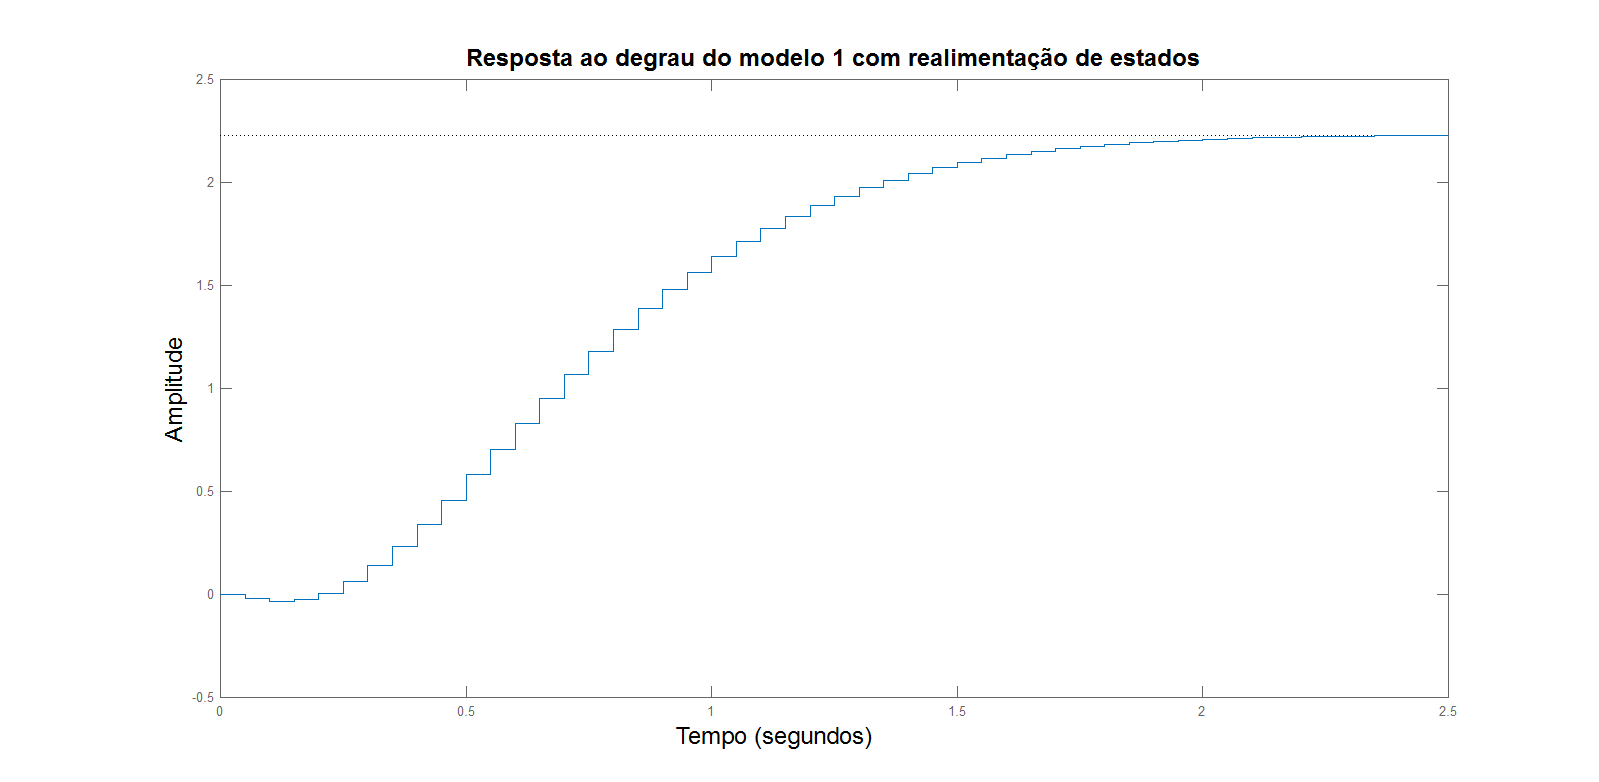
\includegraphics[width=1.1\linewidth]{respostadegraumodelo1realimentacao}
	\caption[Resposta ao degrau do modelo 1 com realimentação de estados]{}
	\caption{Resposta ao degrau do modelo 1 com realimentação de estados}
	\label{fig:respostadegraumodelo1realimentacao}
\end{figure}

A resposta ao degrau do sistema como vista na figura \ref{fig:respostadegraumodelo1realimentacao} apresenta um tempo de assentamento de 1.8 segundos e um sobrevalor de 0.14\%.

\subsection{Modelo 2: Identificado por Mínimos Quadrados}

O modelo 2 vai ter os mesmos requisitos de tempo de assentamento e sobrevalor, mas devido à diferença de ordem entre eles observamos que não conseguimos alocar os polos no mesmo lugar por causa da interação da quantidade de polos. Escolhemos os valores de $\zeta=0.9$ e $\omega_n=10$. Ao aplicar esses valores na equação \eqref{eq:mso} obtemos os polos que precisamos alocar no domínio s, $s_1=0.6225 + 0.1379i$ e $s_2=0.6225 - 0.1379i$, para os polos distantes alocamos $s_3=-14$, $s_4=-14.1$ e $s_5=-14.2$. Que no domínio z são $z_3=0.4966$, $z_4=0.4941$ e $z_5=0.4916$. Repetimos o mesmo procedimento usado para o modelo 1 e obtemos $k=[-1.1768,~2.2245,~-1.1031,~-0.0375,~0.0407]$.


O sistema realimentado tem a seguinte resposta ao degrau:

\begin{figure}[H]
	\centering
	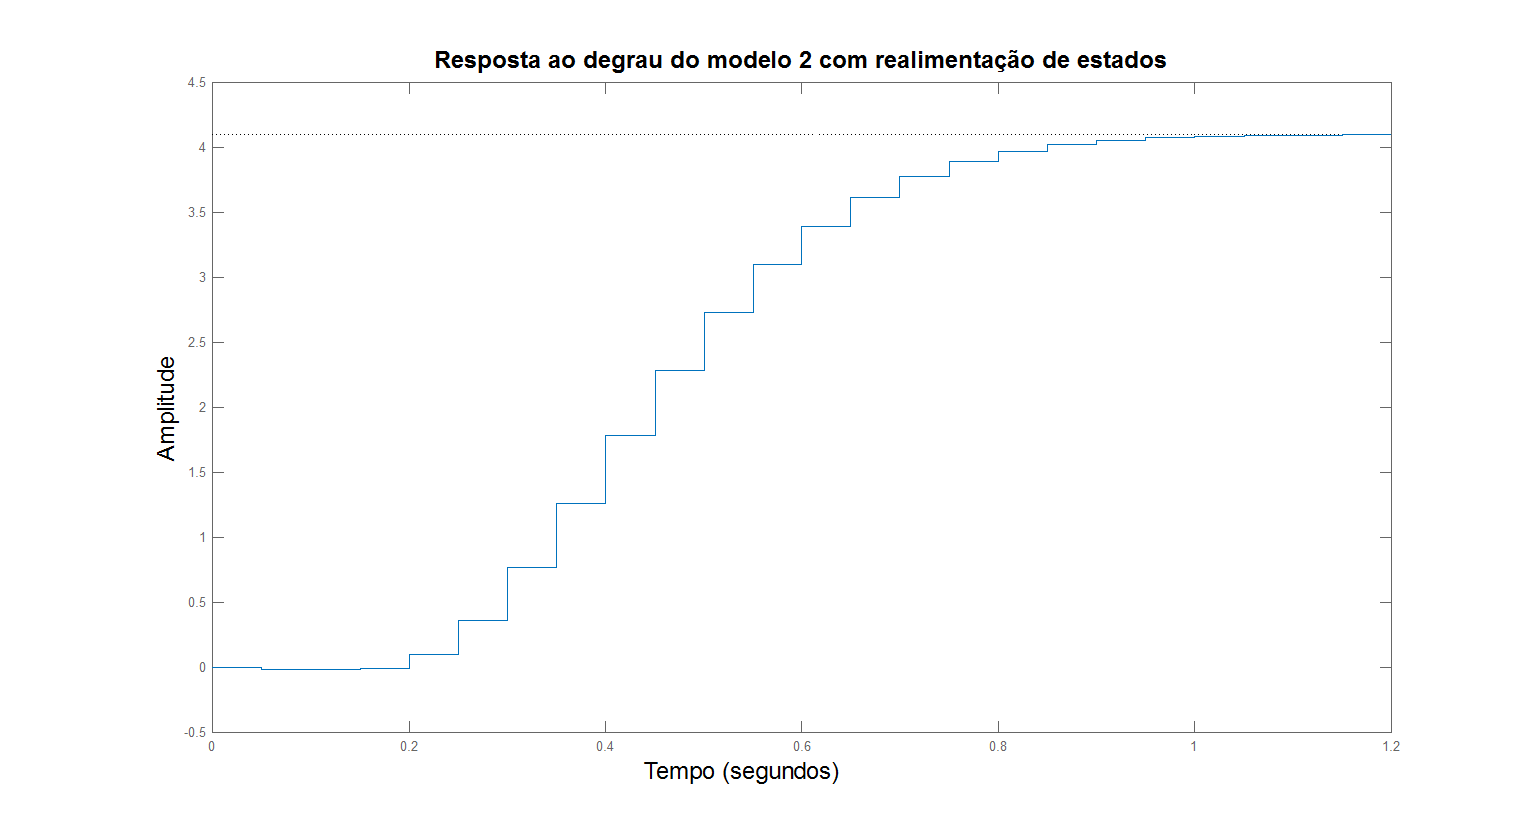
\includegraphics[width=1.1\linewidth]{respostadegraumodelo2realimentacao}
	\caption[Resposta ao degrau do modelo 2 com realimentação de estados]{Resposta ao degrau do modelo 2 com realimentação de estados}
	\label{fig:respostadegraumodelo2realimentacao}
\end{figure}

A resposta ao degrau da figura \ref{fig:respostadegraumodelo2realimentacao} apresenta um tempo de assentamento de 0.85 segundos e um sobrevalor de 0,0165\%. O tempo de assentamento aqui parece mais rápido do que foi constatado no sistema real.

\section{Projeto do Estimador de Estados}
Para realizar um controlador por realimentação de estados precisamos ser capazes de medir todos os estados do nosso modelo a cada tempo de amostragem. O nosso sistema, no entanto, não tem sensores para medir cada um dos estados necessários, a única medida disponível é a saída do sistema na forma da altura da bola. Portanto, precisamos implementar um estimador de estados para cada um dos controladores projetados na subseção anterior.

\subsection{Modelo 1}
Um estimador de estados é projetado de forma similar ao controlador por realimentação de estados, precisamos escolher polos adequados para que o estimador funcione da forma correta. A forma mais simples de escolher esses polos é fazer com que eles reajam mais rápido que o sistema à entrada recebida, conseguimos isso multiplicando a parte real dos polos no domínio s por um número para que sejam mais rápidos. 


Projetamos o estimador de estados com os seguintes polos $z_1=0.2587+0.0169 i$, $z_2=0.2587-0.0169 i$ e $z_3=0.0183$ e obtemos o ganho do estimador $L=[2.4161,~-6.6736,~9.3227]^T$

\subsection{Modelo 2}
Para o estimador do modelo 2 alocamos os polos em $z_1=0.0069 - 0.0015i$, $z_2=0.0069 + 0.0015i$, $z_3=0.0005 + 0.0000i$, $z_4=0.0004 + 0.0000i$ e $z_5=0.0004 + 0.0000i$.




















% Fim Capítulo
